\documentclass{article}
\usepackage{ifthen}
\usepackage{amssymb}
\usepackage{multicol}
\usepackage{graphicx}
\usepackage[absolute]{textpos}
\usepackage{amsmath, amscd, amssymb, amsthm, latexsym}
\usepackage{xspace,rotating,dsfont,ifthen}
\usepackage[spanish,activeacute]{babel}
\usepackage[utf8]{inputenc}
\usepackage{pgfpages}
\usepackage{pgf,pgfarrows,pgfnodes,pgfautomata,pgfheaps,xspace,dsfont}
\usepackage{listings}
\usepackage{multicol}
\usepackage{todonotes}
\usepackage{url}
\usepackage{float}
\usepackage{framed,mdframed}
\usepackage{cancel}

\usepackage[strict]{changepage}


\makeatletter


\newcommand\hfrac[2]{\genfrac{}{}{0pt}{}{#1}{#2}} %\hfrac{}{} es un \frac sin la linea del medio

\newcommand\Wider[2][3em]{% \Wider[3em]{} reduce los m\'argenes
\makebox[\linewidth][c]{%
  \begin{minipage}{\dimexpr\textwidth+#1\relax}
  \raggedright#2
  \end{minipage}%
  }%
}


\@ifclassloaded{beamer}{%
  \newcommand{\tocarEspacios}{%
    \addtolength{\leftskip}{4em}%
    \addtolength{\parindent}{-3em}%
  }%
}
{%
  \usepackage[top=1cm,bottom=2cm,left=1cm,right=1cm]{geometry}%
  \usepackage{color}%
  \newcommand{\tocarEspacios}{%
    \addtolength{\leftskip}{3em}%
    \setlength{\parindent}{0em}%
  }%
}

\usepackage{caratula}
\usepackage{enumerate}
\usepackage{hyperref}
\usepackage{graphicx}
\usepackage{amsfonts}
\usepackage{enumitem}
\usepackage{amsmath}

\decimalpoint
\hypersetup{colorlinks=true, linkcolor=black, urlcolor=blue}
\setlength{\parindent}{0em}
\setlength{\parskip}{0.5em}
\setcounter{tocdepth}{2} % profundidad de indice
\setcounter{section}{5} % nro de section
\renewcommand{\thesubsubsection}{\thesubsection.\Alph{subsubsection}}
\graphicspath{ {images/} }

% End latex config

\begin{document}

\titulo{Práctica 6}
\fecha{2do cuatrimestre 2021}
\materia{Álgebra I}
\integrante{Yago Pajariño}{546/21}{ypajarino@dc.uba.ar}

%Carátula
\maketitle
\newpage

%Indice
\tableofcontents
\newpage

% Aca empieza lo propio del documento
\section{Práctica 6}

\subsection{Ejercicio 1}

\subsubsection{Pregunta i}

Paso a polares:
\begin{itemize}
    \item $ 5i = 5(\cos(\frac{\pi}{2}) + i\sin(\frac{\pi}{2})) $
    \item $ (1+i)^4 = (\sqrt{2})^4 .(\cos(\pi)+i\sin(\pi)) $
\end{itemize}

Luego,
\begin{align*}
    z &= 4.5(\cos(\pi + \frac{\pi}{2})+i\sin(\pi +\frac{\pi}{2})) \\
    &= 20(\cos(\frac{3\pi}{2})+i\sin(\frac{3\pi}{2})) \\
\end{align*}

Así,
\begin{itemize}
    \item $ Re(z) = 20. \cos(\frac{3\pi}{2}) = 0 $
    \item $ Im(z) = 20. \sin(\frac{3\pi}{2}) = -20 $
    \item $ |z| = 20 $
    \item $ Re(z^{-1}) = 0 $
    \item $ iz = 20(\cos(2\pi)+i\sin(2\pi)) \implies Im(iz) = 0 $
\end{itemize}

\subsubsection{Pregunta ii}

\begin{align*}
    z &= (\sqrt[]{2} + \sqrt[]{3}i)^2.(\overline{1-3i}) \\
    &= (2 + 2\cdot \sqrt[]{2} \cdot\sqrt[]{3}i - 3).(1 + 3i) \\
    &= (-1 + 2\cdot \sqrt[]{6}i).(1 + 3i) \\
    &= -1 - 3i + 2 \cdot\sqrt[]{6}i - 6 \cdot \sqrt[]{6} \\
    &= -1 - 6 \cdot \sqrt[]{6} + (2 \cdot\sqrt[]{6} - 3)i \\
\end{align*}

\begin{itemize}
    \item $ Re(z) = -1 - 6 \cdot \sqrt[]{6} $
    \item $ Im(z) = 2 \cdot\sqrt[]{6} - 3 $
    \item $ |z| = \sqrt{(-1 - 6 \cdot \sqrt[]{6})^2 + (2 \cdot\sqrt[]{6} - 3)^2} = \sqrt[]{250} = 5\cdot\sqrt[]{10} $
\end{itemize}

\subsubsection{Pregunta iii}

Paso a polares,

$ i^{17} = \cos(17.\frac{\pi}{2}) + i\sin(17\frac{\pi}{2}) $

$ \frac{1}{2} = \frac{1}{2}.(\cos(0) + i\sin(0)) $

$ i = \cos(\frac{\pi}{2}) +i\sin(\frac{\pi}{2}) $

$ (1-i)^3 = (\sqrt[]{2})^3(\cos(3.\frac{7}{4}\pi)+i\sin(3.\frac{7}{4}\pi)) $

Luego,
\begin{align*}
    \frac{1}{2} . i . (1+i)^3 &= \frac{1}{2}.(\sqrt[]{2})^3.\left(\cos(\frac{\pi}{2} + \frac{21}{4}\pi) +i\sin(\frac{\pi}{2} + \frac{21}{4}\pi)\right) \\
    &= \frac{\sqrt[]{2}^3}{2}.\left(\cos\left(\frac{23}{4}\pi\right) +i\sin\left(\frac{23}{4}\pi\right)\right) \\
\end{align*}
Entonces,
\begin{align*}
    z &= \frac{\sqrt[]{2}^3}{2}.\left(\cos\left((\frac{17}{2} + \frac{23}{4})\pi\right) +i\sin\left((\frac{17}{2} + \frac{23}{4})\pi\right)\right) \\
    &= \frac{\sqrt[]{2}^3}{2}.\left(\cos\left(\frac{57}{4}\pi\right) +i\sin\left(\frac{57}{4}\pi\right)\right) \\
\end{align*}

\begin{itemize}
    \item $ Re(z) = \frac{\sqrt[]{2}^3}{2} . \cos\left(\frac{57}{4}\pi\right) $
    \item $ Im(z) = \frac{\sqrt[]{2}^3}{2} . \sin\left(\frac{57}{4}\pi\right) $
    \item $ |z| = \frac{\sqrt[]{2}^3}{2} $
    \item $ Re(z^{-1}) = \cos\left(\frac{57}{4}\pi\right) $
    \item $ Im(iz) = \frac{\sqrt[]{2}^3}{2} . \sin\left(\frac{59}{4}\pi\right) $
\end{itemize}

\subsubsection{Pregunta iv}
TODO

\subsubsection{Pregunta v}
TODO

\subsection{Ejercicio 2}

\begin{enumerate}
    \item 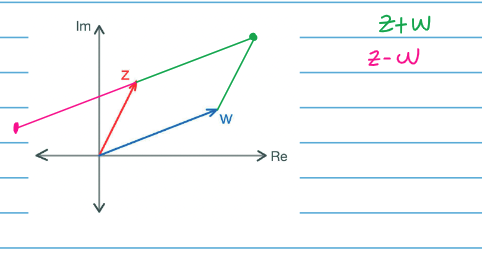
\includegraphics[width=250px]{6.2.1}
    \item 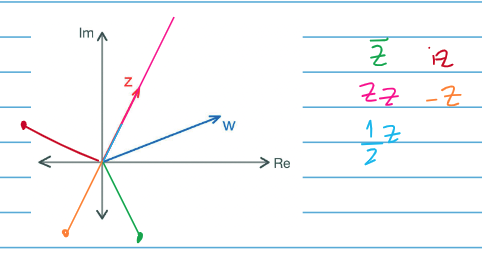
\includegraphics[width=250px]{6.2.2}
    \item 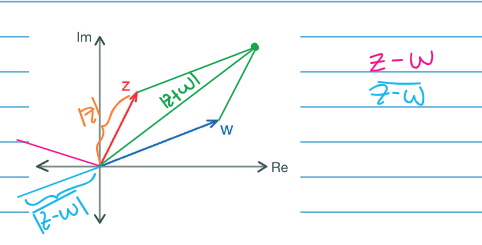
\includegraphics[width=250px]{6.2.3}
\end{enumerate}

\subsection{Ejercicio 3}

\subsubsection{Pregunta i}

$ z^2 = -36 $

Se que $ z = a+bi $ con $ (a,b) \in \mathbb{R}^2 $

Luego busco los $z$ tales que $z^2 = -36 $

\begin{align*}
    z^2 = -36 \iff z^2 &= (a+bi)^2 \\
    &= a^2 - b^2 + 2abi \\
\end{align*}

También se que el módulo debe ser igual $ |z^2| = |-36| $,

$ |z^2| = |z|^2 = (\sqrt{a^2+b^2})^2 = a^2+b^2 $ \\
$ |-36| = 36 $

Usando la igualdad de números complejos,

$ \begin{cases}
    a^2-b^2 = -36 \\
    2ab = 0 \\
    a^2+b^2 = 36 \\
\end{cases} $

Sumando (1) y (3) $ 2a^2 = 0 \iff a = 0 $

Restando (1) a (3) $ 2b^2 = 2.36 \iff b = \pm 36 $

Luego $ z = a+bi $ con los valores de a y b hallados resulta en

Rta.: $ z_1 = 6i; z_2 = -6i $

\subsubsection{Pregunta ii}

$ z^2 = i $

Se que $ z = a+bi $ con $ (a,b) \in \mathbb{R}^2 $

También se que el módulo debe ser igual $ |z^2| = |i| $,

$ |z^2| = |z|^2 = (\sqrt{a^2+b^2})^2 = a^2+b^2 $ \\
$ |i| = 1 $

Usando la igualdad de números complejos,

$ \begin{cases}
    a^2-b^2 = 0 \\
    2ab = 1 \\
    a^2+b^2 = 1 \\
\end{cases} $

Sumando (1) y (3) $ 2a^2 = 1 \iff a = \pm \frac{1}{\sqrt[]{2}} $

Restando (1) a (3) $ 2b^2 = 1 \iff b = \pm \frac{1}{\sqrt[]{2}} $

Usando (2) se que $ 2ab > 0 \iff (a > 0 \wedge b > 0) \vee (a < 0 \wedge b < 0) $

Rta.: $ z_1 = \frac{1}{\sqrt[]{2}} + \frac{1}{\sqrt[]{2}}i; z_2 = -\frac{1}{\sqrt[]{2}} - \frac{1}{\sqrt[]{2}}i $

\subsubsection{Pregunta iii}

$ z^2 = 7+24i $

Se que $ z = a+bi $ con $ (a,b) \in \mathbb{R}^2 $

También se que el módulo debe ser igual $ |z^2| = |7+24i| $,

$ |z^2| = |z|^2 = (\sqrt{a^2+b^2})^2 = a^2+b^2 $

$ |7+24i| = \sqrt[]{7^2+24^2} = \sqrt[]{49+576} = 25 $

Usando la igualdad de números complejos,

$ \begin{cases}
    a^2-b^2 = 7 \\
    2ab = 24 \\
    a^2+b^2 = 25 \\
\end{cases} $

Sumando (1) y (3) $ 2a^2 = 32 \iff a = \pm 4 $

Restando (1) a (3) $ 2b^2 = 18 \iff b = \pm 3 $

Usando (2) se que $ 2ab > 0 \iff (a > 0 \wedge b > 0) \vee (a < 0 \wedge b < 0) $

Rta.: $ z_1 = 4+3i; z_2 = -4-3i $

\subsubsection{Pregunta iv}

$ z^2 + 15 - 8i = 0 \iff z^2 = -15+8i $

Se que $ z = a+bi $ con $ (a,b) \in \mathbb{R}^2 $

También se que el módulo debe ser igual $ |z^2| = |-15+8i| $,

$ |z^2| = |z|^2 = (\sqrt{a^2+b^2})^2 = a^2+b^2 $

$ |-15+8i| = \sqrt[]{(-15)^2+8^2} = \sqrt[]{225 + 64} = 17 $

Usando la igualdad de números complejos,

$ \begin{cases}
    a^2-b^2 = -15 \\
    2ab = 8 \\
    a^2+b^2 = 17 \\
\end{cases} $

Sumando (1) y (3) $ 2a^2 = 2 \iff a = \pm 1 $

Restando (1) a (3) $ 2b^2 = 16 \iff b = \pm 4 $

Usando (2) se que $ 2ab > 0 \iff (a > 0 \wedge b > 0) \vee (a < 0 \wedge b < 0) $

Rta.: $ z_1 = 1+4i; z_2 = -1-4i $

\subsection{Ejercicio 4}

\subsubsection{Pregunta i}

$ z = (2+2i)(\sqrt[]{3}-i) $

Busco la forma polar de cada factor.
\begin{align*}
    2+2i &= \sqrt[]{8}. e^{\frac{\pi}{4}i} \\
    \sqrt[]{3} - i &= 2.e^{\frac{11}{6}\pi i}
\end{align*}
Por DeMoivre,
\begin{align*}
    z &= (2+2i)(\sqrt[]{3}-i) \\
    &= \sqrt[]{8}. 2. e^{\frac{\pi}{4}i + \frac{11}{6}\pi i} \\
    &= 2 \cdot \sqrt[]{8} e^{\frac{1}{12}\pi i}
\end{align*}
Luego,
\begin{itemize}
    \item $ |z| = 4\cdot \sqrt[]{2} $
    \item $ \theta = \frac{1}{12}\pi $
\end{itemize}

\subsubsection{Pregunta ii}

$ z = (-1+\sqrt[]{3}i)^5 $
\begin{align*}
    -1+\sqrt[]{3}i &= 2\cdot e^{(\pi - \frac{1}{3}\pi)i} \\
    &= 2\cdot e^{\frac{2}{3}\pi i } 
\end{align*}
Luego,
\begin{align*}
    z &= (-1+\sqrt[]{3}i)^5 \\
    &= (2\cdot e^{\frac{2}{3}\pi i })^5 \\
    &= 2^5\cdot e^{\frac{10}{3}\pi i }
\end{align*}
Por lo tanto,
\begin{itemize}
    \item $ |z| = 2^5 $
    \item $ \theta = \frac{4}{3}\pi $
\end{itemize}

\subsubsection{Pregunta iii}

$ z = (-1+\sqrt[]{3}i)^{-5} $
\begin{align*}
    z &= (-1+\sqrt[]{3}i)^{-5} \\
    &= (2\cdot e^{\frac{2}{3}\pi i })^{-5} \\
    &= 2^{-5}\cdot e^{\frac{-10}{3}\pi i }
\end{align*}
Por lo tanto,
\begin{itemize}
    \item $ |z| = \frac{1}{2^5} $
    \item $ \theta = \frac{2}{3}\pi $
\end{itemize}

\subsubsection{Pregunta iv}

$ z = \frac{1+\sqrt[]{3}i}{1-i} $

Busco las expresiones polares.
\begin{align*}
    1+\sqrt[]{3}i &= 2. e^{\frac{\pi}{3}i} \\
    1-i &= \sqrt[]{2}. e^{\frac{7}{4}\pi i}
\end{align*}
Luego,
\begin{align*}
    z &= \frac{1+\sqrt[]{3}i}{1-i} \\
    &= \frac{2}{\sqrt[]{2}} \cdot e^{(\frac{1}{3} - \frac{7}{4})\pi i} \\
    &= \frac{2}{\sqrt[]{2}} \cdot e^{\frac{-17}{12}\pi i}
\end{align*}
Por lo tanto,
\begin{itemize}
    \item $ |z| = \frac{2}{\sqrt[]{2}} $
    \item $ \theta = \frac{7}{12}\pi $
\end{itemize}

\subsection{Ejercicio 5}

\subsubsection{Pregunta i}

$ Re(z) = x \wedge Im(z) = y \implies x+5y \leq 8 \iff y \leq -\frac{1}{5}x + \frac{8}{5}$

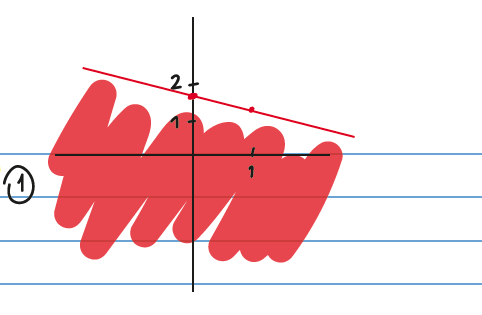
\includegraphics[width=250px]{6.5.1}

\subsubsection{Pregunta ii}

\begin{itemize}
    \item $ |z| = 2 $ define una circunferencia de radio 2.
    \item $ \frac{\pi}{4} \leq arg(z) \leq \frac{2\pi}{3} $ define un arco de angulo barrido.
\end{itemize}

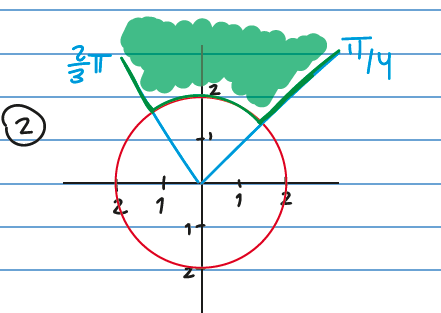
\includegraphics[width=250px]{6.5.2}

\subsubsection{Pregunta iii}
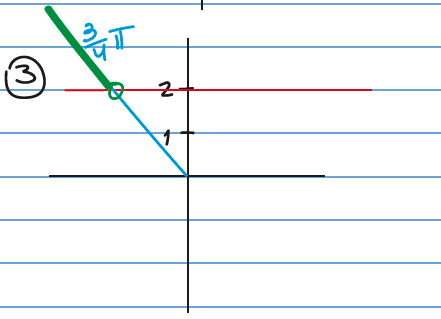
\includegraphics[width=250px]{6.5.3}

\subsubsection{Pregunta iv}
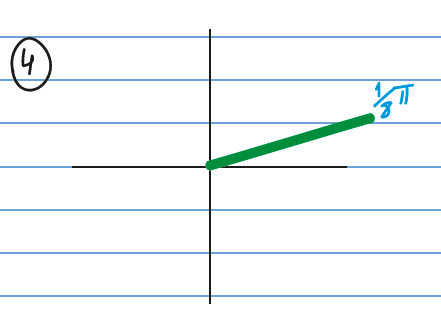
\includegraphics[width=250px]{6.5.4}

\subsection{Ejercicio 6}

\subsubsection{Pregunta i}

$ z = (\frac{1+\sqrt[]{3}i}{1-i})^{17} $

Sea $ w = \frac{1+\sqrt[]{3}i}{1-i} $

Busco las expresiones polares.
\begin{align*}
    1+\sqrt[]{3}i &= 2. e^{\frac{\pi}{3}i} \\
    1-i &= \sqrt[]{2}. e^{\frac{7}{4}\pi i}
\end{align*}
Luego,
\begin{align*}
    w &= \frac{1+\sqrt[]{3}i}{1-i} \\
    &= \frac{2}{\sqrt[]{2}} \cdot e^{(\frac{1}{3} - \frac{7}{4})\pi i} \\
    &= \frac{2}{\sqrt[]{2}} \cdot e^{\frac{7}{12}\pi i}
\end{align*}
Por lo tanto,
\begin{align*}
    z &= w^{17} \\
    &= \left(\frac{2}{\sqrt[]{2}} \cdot e^{\frac{7}{12}\pi i}\right)^{17} \\
    &= \left(\frac{2}{\sqrt[]{2}}\right)^{17} \cdot e^{\frac{17.7}{12}\pi i} \\
    &= \left(\frac{2}{\sqrt[]{2}}\right)^{17} \cdot e^{\frac{23}{12}\pi i} \\
\end{align*}
Por lo tanto,
$ z = \left(\frac{2}{\sqrt[]{2}}\right)^{17} \cdot \cos(\frac{23}{12}\pi i) + \left(\frac{2}{\sqrt[]{2}}\right)^{17} \cdot \sin(\frac{23}{12}\pi i) $

\subsubsection{Pregunta ii}

$ z = (-1+\sqrt[]{3}i)^{n} $

$ -1+\sqrt[]{3}i = 2\cdot e^{\frac{2}{3}\pi i} $

$ (-1+\sqrt[]{3}i)^{n} = 2^n \cdot e^{\frac{2n}{3}\pi i} $

Luego $ 0 \leq \frac{2n}{3}\pi i < 2\pi \iff 0 \leq n < 3 $

Por lo tanto,
\begin{itemize}
    \item $ n = 0 \implies z = 1 $
    \item $ n = 1 \implies z = 2\cdot e^{\frac{2}{3}\pi i} = -1+\sqrt[]{3}i $
    \item $ n = 1 \implies z = 4\cdot e^{\frac{4}{3}\pi i} = -2+ 2 \cdot \sqrt[]{3}i $
\end{itemize}

\subsection{Ejercicio 7}

\subsubsection{Pregunta i}

Busco los $ n \in \mathbb{N} $ tales que $ (\sqrt[]{3}-i)^n = 2^{n-1}\cdot (-1+\sqrt[]{3}i) $

Luego,
\begin{align*}
    (\sqrt[]{3}-i)^n = 2^{n-1}\cdot (-1+\sqrt[]{3}i) &\iff 2(\sqrt[]{3}-i)^n = 2^{n}\cdot (-1+\sqrt[]{3}i) \\
    &\iff \left(\frac{\sqrt[]{3}-i}{2}\right)^n = \frac{-1+\sqrt[]{3}i}{2} \\
\end{align*}
Busco expresiones polares,
\begin{itemize}
    \item $ -1+\sqrt[]{3}i = 2\cdot e^{\frac{2}{3}\pi i} $
    \item $ 2 = 2\cdot e^{0} $
    \item $ \sqrt[]{3}-i = 2\cdot e^{\frac{11}{6}\pi i} $
\end{itemize}
Así,
\begin{align*}
    \frac{-1+\sqrt[]{3}i}{2} &= 1\cdot e^{\frac{2}{3}\pi i} \\
    &= e^{\frac{2}{3}\pi i} \\
\end{align*}
Y,
\begin{align*}
    \frac{\sqrt[]{3}-i}{2} &= 1\cdot e^{\frac{11}{6}\pi i} \\
    &= e^{\frac{11}{6}\pi i} \\
    \implies \left(\frac{\sqrt[]{3}-i}{2}\right)^n &= e^{\frac{11}{6}n\pi i}
\end{align*}

Luego sea $ z = e^{\frac{2}{3}\pi i} $ y $ w = e^{\frac{11}{6}n\pi i} $ por definición de números complejos,
$
    z = w \iff \begin{cases}
        |z| = |w| \\
        \frac{2}{3}\pi = \frac{11}{6}n\pi +2k\pi
    \end{cases}
$

Luego,
\begin{align*}
    \frac{2}{3}\pi &= \frac{11}{6}n\pi +2k\pi \\
    \frac{2}{3} &= \frac{11}{6}n +2k \\
    4 &= 11n + 12k \\
    11n &= - 12k + 4 \\
    \iff 11n &\equiv 4(12) \\
    -n &\equiv 4(12) \\
    n &\equiv 8(12) \\
\end{align*}
Rta.: $ w = z \iff n \equiv 8(12) $

\subsubsection{Pregunta ii}

Busco los $ n \in \mathbb{N} $ tales que $ (-\sqrt[]{3}+i)^n \cdot \left(\frac{1}{2} + \frac{\sqrt[]{3}}{2}\right) $ es un real negativo

Busco expresiones polares.

\begin{itemize}
    \item $ -\sqrt[]{3}+i = 2\cdot e^{\frac{5}{6} \pi i} $
    \item $ \left(\frac{1}{2} + \frac{\sqrt[]{3}}{2}\right) = \left(\frac{1}{2} + \frac{\sqrt[]{3}}{2}\right) \cdot e^0 $
\end{itemize}

Luego,
$ z = 2^n \cdot \left(\frac{1}{2} + \frac{\sqrt[]{3}}{2}\right) \cdot e^{\frac{5}{6} \pi n i} $

Por definición de la forma polar, $ z \in \mathbb{R}_{<0} \iff arg(z) = \pi $

Así,
\begin{align*}
    \frac{5}{6} \pi n &= \pi + 2k \pi \\ 
    \frac{5}{6} n &= 1 + 2k \\ 
    5 n &= 6 + 12k \\ 
    \iff 5.5 n &\equiv 5.6(12) \\ 
    \iff n &\equiv 6(12) \\ 
\end{align*}
Rta.: z es real negativo $ \forall n \in \mathbb{N}: n \equiv 6(12) $

\subsubsection{Pregunta iii}

Busco los $ n \in \mathbb{N} $ tales que $ arg((-1+i)^{2n}) = \frac{\pi}{2} $ y $ arg((1-\sqrt[]{3}i)^{n-1}) = \frac{2}{3}\pi $

Busco expresiones polares.

\begin{itemize}
    \item $ (1-i) = \sqrt[]{2} \cdot e^{\frac{3}{4}\pi i}$
    \item $ (1-i)^{2n} = \left(\sqrt[]{2}\right)^{2n} \cdot e^{2n\frac{3}{4}\pi i} = 2^n \cdot e^{\frac{3}{2}\pi n i} $
    \item $ (1-\sqrt[]{3}i) = 2\cdot e^{\frac{5}{3}\pi i} $
    \item $ (1-\sqrt[]{3}i)^{n-1} = 2^{n-1}\cdot e^{(n-1)\frac{5}{3}\pi i} $
\end{itemize}

Luego resolviendo la primer igualdad,
\begin{align*}
    arg((-1+i)^{2n}) = \frac{\pi}{2} \iff \frac{3}{2}\pi n &= \frac{\pi}{2} + 2k\pi \\ 
    \frac{3}{2} n &= \frac{1}{2} + 2k \\ 
    3 n &= 1 + 4k \\ 
    3 n &\equiv 1 (4) \\ 
    n &\equiv 3 (4) \\ 
\end{align*}
Y la segunda,
\begin{align*}
    arg((1-\sqrt[]{3}i)^{n-1}) = \frac{2}{3}\pi \iff (n-1)\frac{5}{3}\pi &= \frac{2}{3} \pi + 2k\pi \\  
    (n-1)\frac{5}{3} &= \frac{2}{3} + 2k \\  
    (n-1)5 &= 2 + 6k \\  
    5n-5 &= 2 + 6k \\  
    5n &= 7 + 6k \\  
    5n &\equiv 7 (6) \\  
    -n &\equiv 7 (6) \\  
    n &\equiv 5 (6) \\  
\end{align*}

Juntando ambas soluciones, $ \begin{cases}
    n \equiv 3(4) \implies n \equiv 1(2) \\
    n \equiv 5(6)
\end{cases} $

La segunda implica la primera, luego los n que cumplen lo pedido son $ \{ n \in \mathbb{N}: n\equiv 5(6) \} $

\subsection{Ejercicio 8}

\subsubsection{Pregunta i}

Busco los $ w: w^6 = 8 $

Se que, $ \begin{cases}
    8 = 8 \cdot e^0 \\
    w^6 = |w|^6 \cdot e^{6 \theta i}
\end{cases} $

Luego por igualdad de números complejos, $ w^6 = 8 \iff \begin{cases}
    |w|^6 = 8 \\
    \theta = \frac{0+2k\pi}{6}
\end{cases} $

Con $ 0 \leq \theta < 2\pi \iff 0 \leq \frac{k\pi}{3} < 2\pi \iff 0 \leq k < 6 \implies k \in \{ 0,1,2,3,4,5 \} $

Así, las raíces sextas de 8 son:
\begin{itemize}
    \item $ n = 0 \implies w_0 = \sqrt[6]{8} \cdot e^0 $
    \item $ n = 1 \implies w_1 = \sqrt[6]{8} \cdot e^{\frac{2}{6} \cdot \pi i} $
    \item $ n = 2 \implies w_2 = \sqrt[6]{8} \cdot e^{\frac{4}{6} \cdot \pi i} $
    \item $ n = 3 \implies w_3 = \sqrt[6]{8} \cdot e^{\frac{6}{6} \cdot \pi i} $
    \item $ n = 4 \implies w_4 = \sqrt[6]{8} \cdot e^{\frac{8}{6} \cdot \pi i} $
    \item $ n = 4 \implies w_5 = \sqrt[6]{8} \cdot e^{\frac{10}{6} \cdot \pi i} $
\end{itemize}

\subsubsection{Pregunta ii}

Busco los $ w: w^3 = -4 $

Se que, $ \begin{cases}
    -4 = 4 \cdot e^{\pi i} \\
    w^3 = |w|^3 \cdot e^{3 \theta i}
\end{cases} $

Luego por igualdad de números complejos, $ w^3 = -4 \iff \begin{cases}
    |w|^3 = 4 \implies |w| = \sqrt[3]{4} \\
    \theta = \frac{\pi+2k\pi}{3}
\end{cases} $

Con $ 0 \leq \theta < 2\pi \iff 0 \leq \frac{\pi+2k\pi}{3} < 2\pi \iff 0 \leq k < 3 \implies k \in \{ 0,1,2 \} $

Así, las raíces cubicas de -4 son:
\begin{itemize}
    \item $ n = 0 \implies w_0 = \sqrt[3]{4} \cdot e^{\frac{1}{3} \pi i} $
    \item $ n = 1 \implies w_1 = \sqrt[3]{4} \cdot e^{\pi i} $
    \item $ n = 2 \implies w_2 = \sqrt[3]{4} \cdot e^{\frac{5}{3} \pi i} $
\end{itemize}

\subsubsection{Pregunta iii}

Busco los $ w: w^7 = -1+i $

Se que, $ \begin{cases}
    -1+i = \sqrt[]{2} \cdot e^{\frac{3}{4}\pi i} \\
    w^7 = |w|^7 \cdot e^{7 \theta i}
\end{cases} $

Luego por igualdad de números complejos, $ w^7 = -1+i \iff \begin{cases}
    |w|^7 = \sqrt[]{2} \implies |w| = \sqrt[14]{2} \\
    \theta = \frac{3/4\pi+2k\pi}{7}
\end{cases} $

Con $ 0 \leq \theta < 2\pi \iff 0 \leq \frac{3/4\pi+2k\pi}{7} < 2\pi \iff 0 \leq k < 7 \implies k \in \{ 0,1,2,3,4,5,6 \} $

Así, las raíces séptimas de $ -1+i $ son:
\begin{itemize}
    \item $ n = 0 \implies w_0 = \sqrt[14]{2} \cdot e^{\frac{3}{28} \pi i} $
    \item $ n = 1 \implies w_1 = \sqrt[14]{2} \cdot e^{\frac{11}{28} \pi i} $
    \item $ n = 2 \implies w_2 = \sqrt[14]{2} \cdot e^{\frac{19}{28} \pi i} $
    \item $ n = 3 \implies w_3 = \sqrt[14]{2} \cdot e^{\frac{27}{28} \pi i} $
    \item $ n = 4 \implies w_4 = \sqrt[14]{2} \cdot e^{\frac{35}{28} \pi i} $
    \item $ n = 5 \implies w_5 = \sqrt[14]{2} \cdot e^{\frac{43}{28} \pi i} $
    \item $ n = 6 \implies w_6 = \sqrt[14]{2} \cdot e^{\frac{51}{28} \pi i} $
\end{itemize}

\subsection{Ejercicio 9}

Busco todos los $ z \in \mathbb{C} $ tales que $ 3z^5 + 2|z|^5 + 32 = 0 $

Pero, $ 3z^5 + 2|z|^5 + 32 = 0 \iff 3z^5 = -2|z|^5 - 32 $

Luego por igualdad de números complejos, $ arg(3z^5) = arg(-2|z|^5-32) $
\begin{align*}
    arg(3z^5) &= arg(-2|z|^5-32) \\
    arg(3z^5) &= arg(-2(|z|^5-16)) \\
    arg(3) + arg(z^5) &= arg(-2) + arg(|z|^5-16) + 2k\pi \\
    0 + 5\theta &= \pi + 0 + 2k\pi \\
    \theta &= \frac{\pi}{5} + \frac{2k\pi}{5} \\
\end{align*}
Con $ 0 \leq \frac{\pi}{5} + \frac{2k\pi}{5} < 2\pi \iff 0 \leq 1+2k <10 \iff \frac{-1}{2} \leq k \leq \frac{9}{2} \implies k \in \{0,1,2,3,4\}$

Ahora busco $ |z| $
\begin{align*}
    |3||z|^5 &= |-2|||z|^5 - 16| \\
    3|z|^5 &= 2|z|^5 + 32 \\
    |z|^5 &= 32 \\
    |z| &= \sqrt[5]{32} \\
    |z| &= 2 \\
\end{align*}
Luego $ z = 2 \cdot e^{\theta i} = 2 \cdot e^{\frac{\pi}{5} + \frac{2k\pi}{5}} $ con $ k \in \{0,1,2,3,4\} $

Los z que cumplen lo pedido son:
\begin{itemize}
    \item $ k = 0 \implies z_0 = 2 \cdot e^{\frac{1}{5}\pi i} $
    \item $ k = 1 \implies z_1 = 2 \cdot e^{\frac{3}{5}\pi i} $
    \item $ k = 2 \implies z_2 = 2 \cdot e^{\pi i} $
    \item $ k = 3 \implies z_3 = 2 \cdot e^{\frac{7}{5}\pi i} $
    \item $ k = 4 \implies z_4 = 2 \cdot e^{\frac{9}{5}\pi i} $
\end{itemize}

\subsection{Ejercicio 10}

$ z^n + i\overline{z}^2 = 0 \iff z^n = - i\overline{z}^2$

Voy a usar la igualdad de complejos en forma polar, no cubre el caso $ z = 0 $ asi que lo pruebo primero como caso aparte.

$ z = 0 \implies 0^n + i 0^2 = 0 $ luego tengo la primer solución en $ z = 0 $.

Se que z es de la forma: $ z = |z|\cdot e^{\theta i} $ con $ 0 \leq \theta < 2\pi $

Luego,
\begin{align*}
    \overline{z} &= |z|\cdot e^{-\theta i} \\
    \overline{z}^2 &= |z|^2 \cdot e^{-2 \theta i} \\
    -i\overline{z}^2 &= |z|^2 \cdot e^{\left(-2 \theta + \frac{3}{2}\pi\right) i}
\end{align*}
Por lo tanto, 
\begin{align*}
    z^n &= |z|^2 \cdot e^{\left(-2 \theta + \frac{3}{2}\pi\right) i} \\
    |z|^n\cdot e^{n\theta i} &= |z|^2 \cdot e^{\left(-2 \theta + \frac{3}{2}\pi\right) i} \\
\end{align*}
Por igualdad de números complejos,
\begin{align*}
    |z|^n\cdot e^{n\theta i} &= |z|^2 \cdot e^{\left(-2 \theta + \frac{3}{2}\pi\right) i} \iff  \begin{cases}
        |z|^n = |z|^2 \\
        n\theta = -2 \theta + \frac{3}{2}\pi + 2k\pi
    \end{cases}
\end{align*}
Entonces, mirando la igualdad de los módulos, si $ n = 2 $ existen infinitas soluciones, no sirve pues solo quiero seis.
Pero si $ n \neq 2 \implies |z| = 1$ es la unica solución posible, es el unico número que elevado a dos potencias distintas cualquiera, sigue siendo el mismo.

Ahora busco $ \theta $,
\begin{align*}
    n\theta &= -2 \theta + \frac{3}{2}\pi + 2k\pi \\
    n\theta + 2 \theta &= \frac{3}{2}\pi + 2k\pi \\
    (n+2)\theta &= \frac{3}{2}\pi + 2k\pi \\
    \theta &= \frac{3}{2(n+2)}\pi + \frac{2k}{(n+2)}\pi \\
\end{align*}
Con $ 0 \leq \theta < 2\pi $,
\begin{align*}
    0 &\leq \frac{3}{2(n+2)}\pi + \frac{2k}{(n+2)}\pi < 2\pi \\
    0 &\leq \frac{3}{2(n+2)} + \frac{2k}{(n+2)} < 2 \\
    0 &\leq 3 + 4k < 4(n+2) \\
    0 &\leq 3 + 4k < 4n+8 \\
    -\frac{3}{4} &\leq k < n + \frac{5}{4} \iff k \in \{ 0,1,...,n+1 \}
\end{align*}

Busco cinco soluciones, por lo tanto $ k \in \{ 0,1,2,3,4 \} $

Así las seis soluciones son:
\begin{itemize}
    \item $ k = 0 \implies z_0 = e^{\frac{3}{10}\pi i}$
    \item $ k = 1 \implies z_1 = e^{\frac{7}{10}\pi i}$
    \item $ k = 2 \implies z_2 = e^{\frac{11}{10}\pi i}$
    \item $ k = 3 \implies z_3 = e^{\frac{15}{10}\pi i}$
    \item $ k = 4 \implies z_4 = e^{\frac{19}{10}\pi i}$
    \item $ z_5 = 0 $
\end{itemize}

\subsection{Ejercicio 11}

\subsubsection{Pregunta i}

Se que $ w \in G_7 $
\begin{align*}
    &w + \overline{w} + (w + w^2)^2 - w^{38}(1-w^2) \\
    = &w + \overline{w} + w^2 + 2ww^2 + w^4 - w^{38}-w^{40} \\
    = &w + \overline{w} + w^2 + 2w^3 + w^4 - w^3 + w^5 \\
    = 1+ &w + w^6 + w^2 + w^3 + w^4 + w^5 -1 = \begin{cases}
        -1 & w \neq 1 \\
        6 & w = 1
    \end{cases} \\
\end{align*}

\subsubsection{Pregunta ii}

Se que $ w \in G_3 $
\begin{align*}
    &w^{73} + \overline{w}w^9 + 8 \\
    = &w + w^2w^0 + 8 \\
    = &w + w^2 + 8 \\
    = 1+&w + w^2 + 7 = \begin{cases}
        10 & w = 1 \\
        7 & w \neq 1 \\
    \end{cases} 
\end{align*}

\subsubsection{Pregunta iii}

Se que $ w \in G_10 $
\begin{align*}
    S &= 1 + w^2 + w^{-2} + w^4 + w^{-4} \\
    S &= 1 + w^2 + w^8 + w^4 + w^6 \\
\end{align*}
Si llamo $ z = w^2 \implies z \in G_5 $

Luego,
\begin{align*}
    S = 1 + z + z^4 + z^2 + z^3 = \begin{cases}
        5 & z = 1 \\
        0 & z \neq 1 \\
    \end{cases}
\end{align*}
Pero $ z = w^2 \implies z = 1 \iff w = \pm 1 \implies S = \begin{cases}
    5 & w = \pm 1 \\
    0 & w \neq \pm 1 \\
\end{cases} $

\subsubsection{Pregunta iv}

Se que $ w \in G_5 $
\begin{align*}
    &w^{14} + w^{-8} + \overline{w}^4 + \overline{w^{-3}} \\
    = &w^4 + w^2 + w + w^3 \\
    = 1 + &w^4 + w^2 + w + w^3 -1 = \begin{cases}
        4 & w = 1 \\
        -1 & w \neq 1
    \end{cases}\\
\end{align*}

\subsection{Ejercicio 12}

\subsubsection{Pregunta i}

Se que $ w \in G_{36} \implies w^{36} = 1 $

Si defino $ z = w^4 $ entonces,
\begin{align*}
    \sum_{k = 7}^{60}w^{4k} &= \sum_{k = 0}^{60}z^k - \sum_{k = 0}^{6}z^k \\
    &= \frac{z^{61} - 1}{z-1} - \frac{z^7-1}{z-1} \\
    &= \frac{z^{61} - z^7}{z-1} \\
    &= \frac{z^7(z^{54} - 1)}{z-1} \\
    &= \frac{(w^4)^7((w^4)^{54} - 1)}{w^4-1} \\
    &= \frac{w^{28}((w^{36})^6 - 1)}{w^4-1} \\
    &= \frac{w^{28}(1 - 1)}{w^4-1} \\
    &= 0 \\
\end{align*}

\subsubsection{Pregunta ii}

Por propiedades de los números complejos se que $ Re(z) = \frac{z+\overline{z}}{2} $

Luego,
\begin{align*}
    Re(\sum_{k = 0}^{60}w^k) &= \frac{\sum_{k = 0}^{60}w^k + \sum_{k = 0}^{60}\overline{w}^k}{2} \\
    &= \frac{\frac{w^{61} - 1}{w-1} + \frac{\overline{w}^{61} - 1}{\overline{w}-1}}{2} \\
    &= \frac{\frac{w^{6} - 1}{w-1} + \frac{\overline{w}^{5} - 1}{\overline{w}-1}}{2} \\
    &= \frac{(w^{6} - 1)(\overline{w}-1) + (\overline{w}^{5} - 1)(w-1)}{2(w-1)(\overline{w}-1)} \\
    &= \frac{(w^6-1)(w^{10}-1) + (w^5-1)(w-1)}{2(w-1)(w^{10}-1)} \\
    &= \frac{w^{16} - w^6 - w^{10} + 1 + w^6 - w^5 - w + 1}{2(w^{11} - w^{10} - w + 1)} \\
    &= \frac{- w^{10}- w + 2}{2(- w^{10} - w + 2)} \\
    &= \frac{1}{2} \\
\end{align*}

\subsection{Ejercicio 13}
TODO

\subsection{Ejercicio 14}
TODO

\subsection{Ejercicio 15}
TODO

\end{document}
